\section{\label{sec5}Dataset}
The X-ray survey was performed twice, in 2017 and 2018.  In 2017,
single channel trigger used due to limited readout capacity of
DAQ was susceptible to coherent noise and cosmic backgrounds. As a
result, signal to background ratio of $\sim$1 was attained.  The
following year an upgraded DAQ with full waveform data facilitated a
more complex trigger capable of identifying
cosmic rays and noise events, which improved the signal to backgorund ratio
to 12.

The X-rays are absorbed by the magnetic coils (in COBRA) and the
liquid Xe scintillator.  Monte Carlo simulation of the magnet
estimated the absorption of 70\% and was confirmed by LYSO
scintillator crystals placed inside and outside the magnet in the path
of the X-rays (Figure~\ref{fig:absorption}). The absorption in the
calorimeter due to liquid Xe is dependent on the X-ray absorption
length in Xe ($\lambda_{\mathrm{Xe}}$ = 2.9 mm) and the radial
thickness of Xe column traversed by the X-ray before showering.  The
installation of the MPPCs on the cryostat wall makes it unlikely that
any liquid Xe can accumulate behind the MPPCs\cite{megdesign}.
Therefore, loss in signal due to such interactions is expected to be
small.  The normalized rate of X-ray decays observed as a function of
radial distance is shown in figure~\ref{fig:absorption}.

\begin{figure}[]
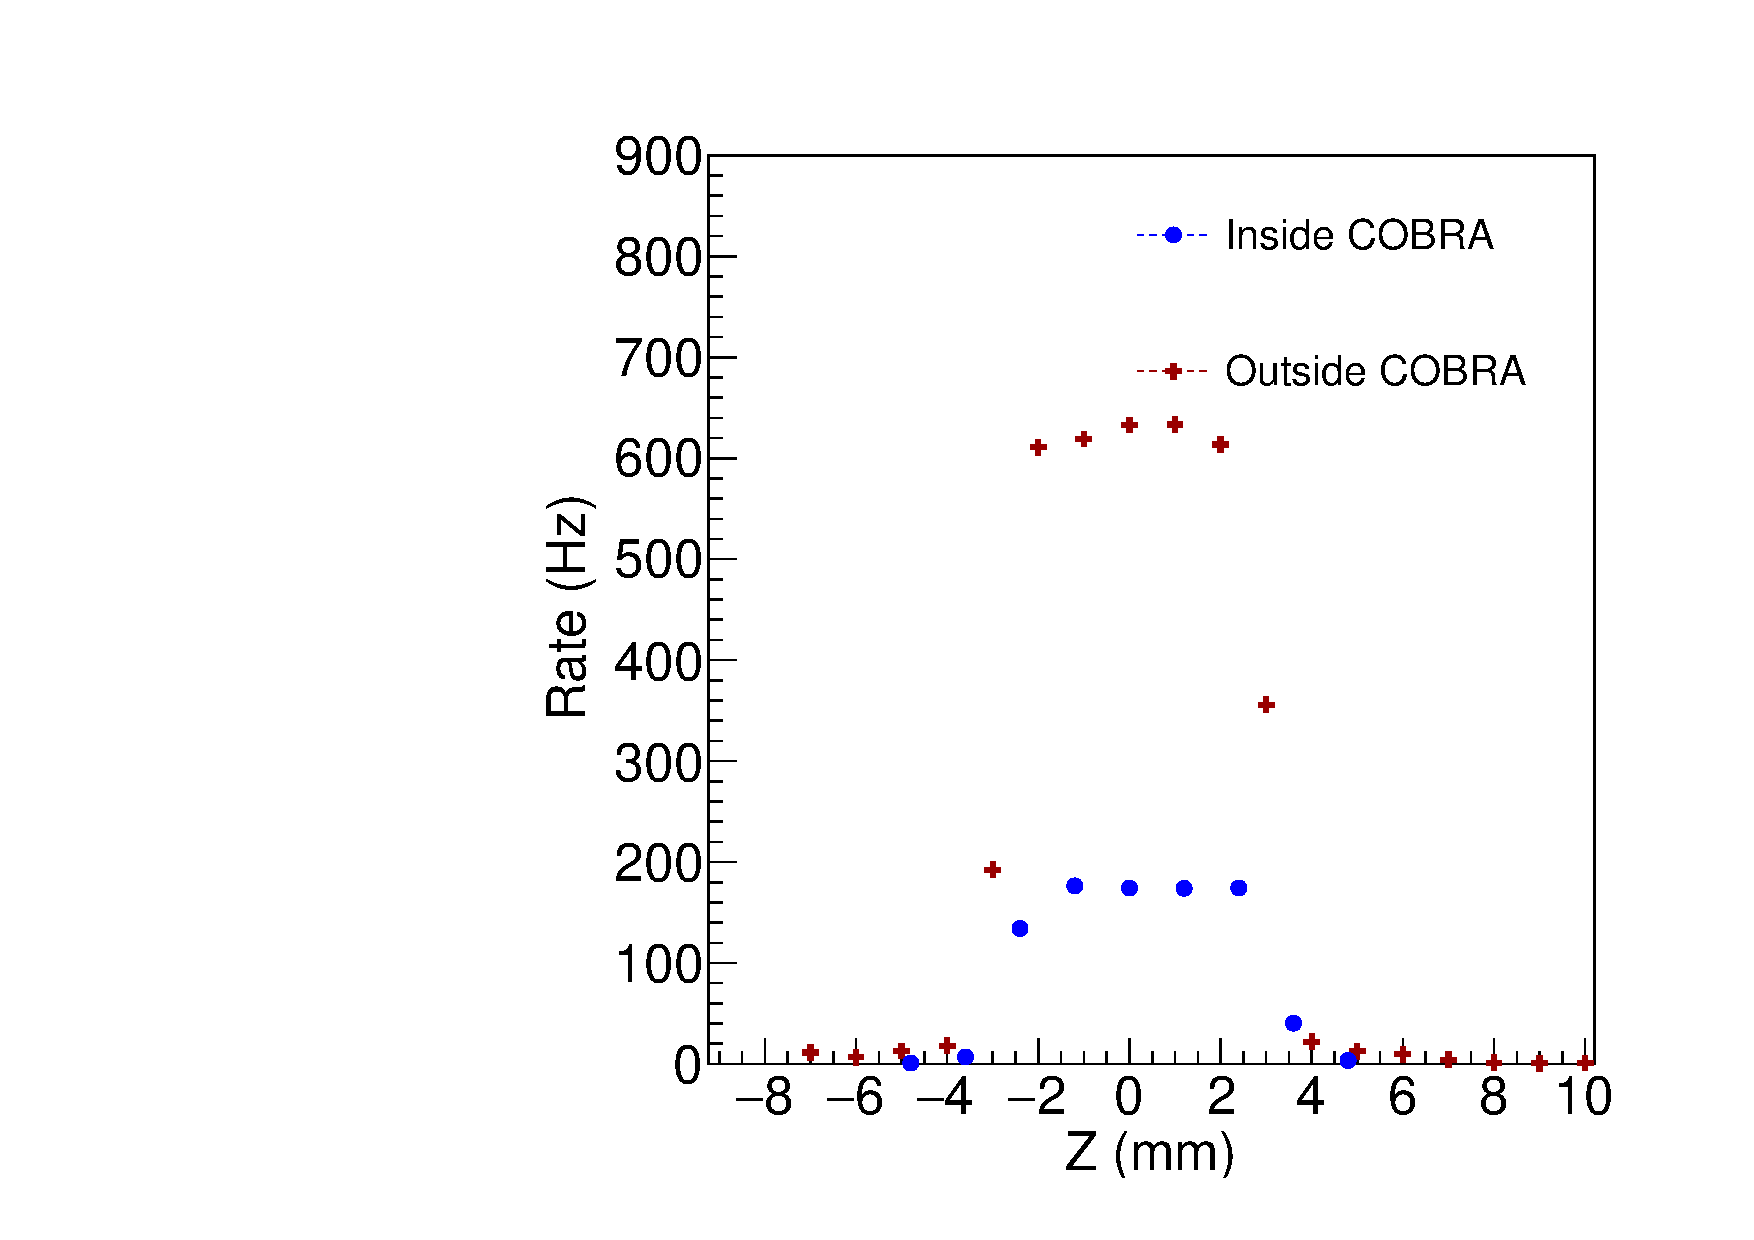
\includegraphics[width=4cm]{plots/xray_cobra_absorption}
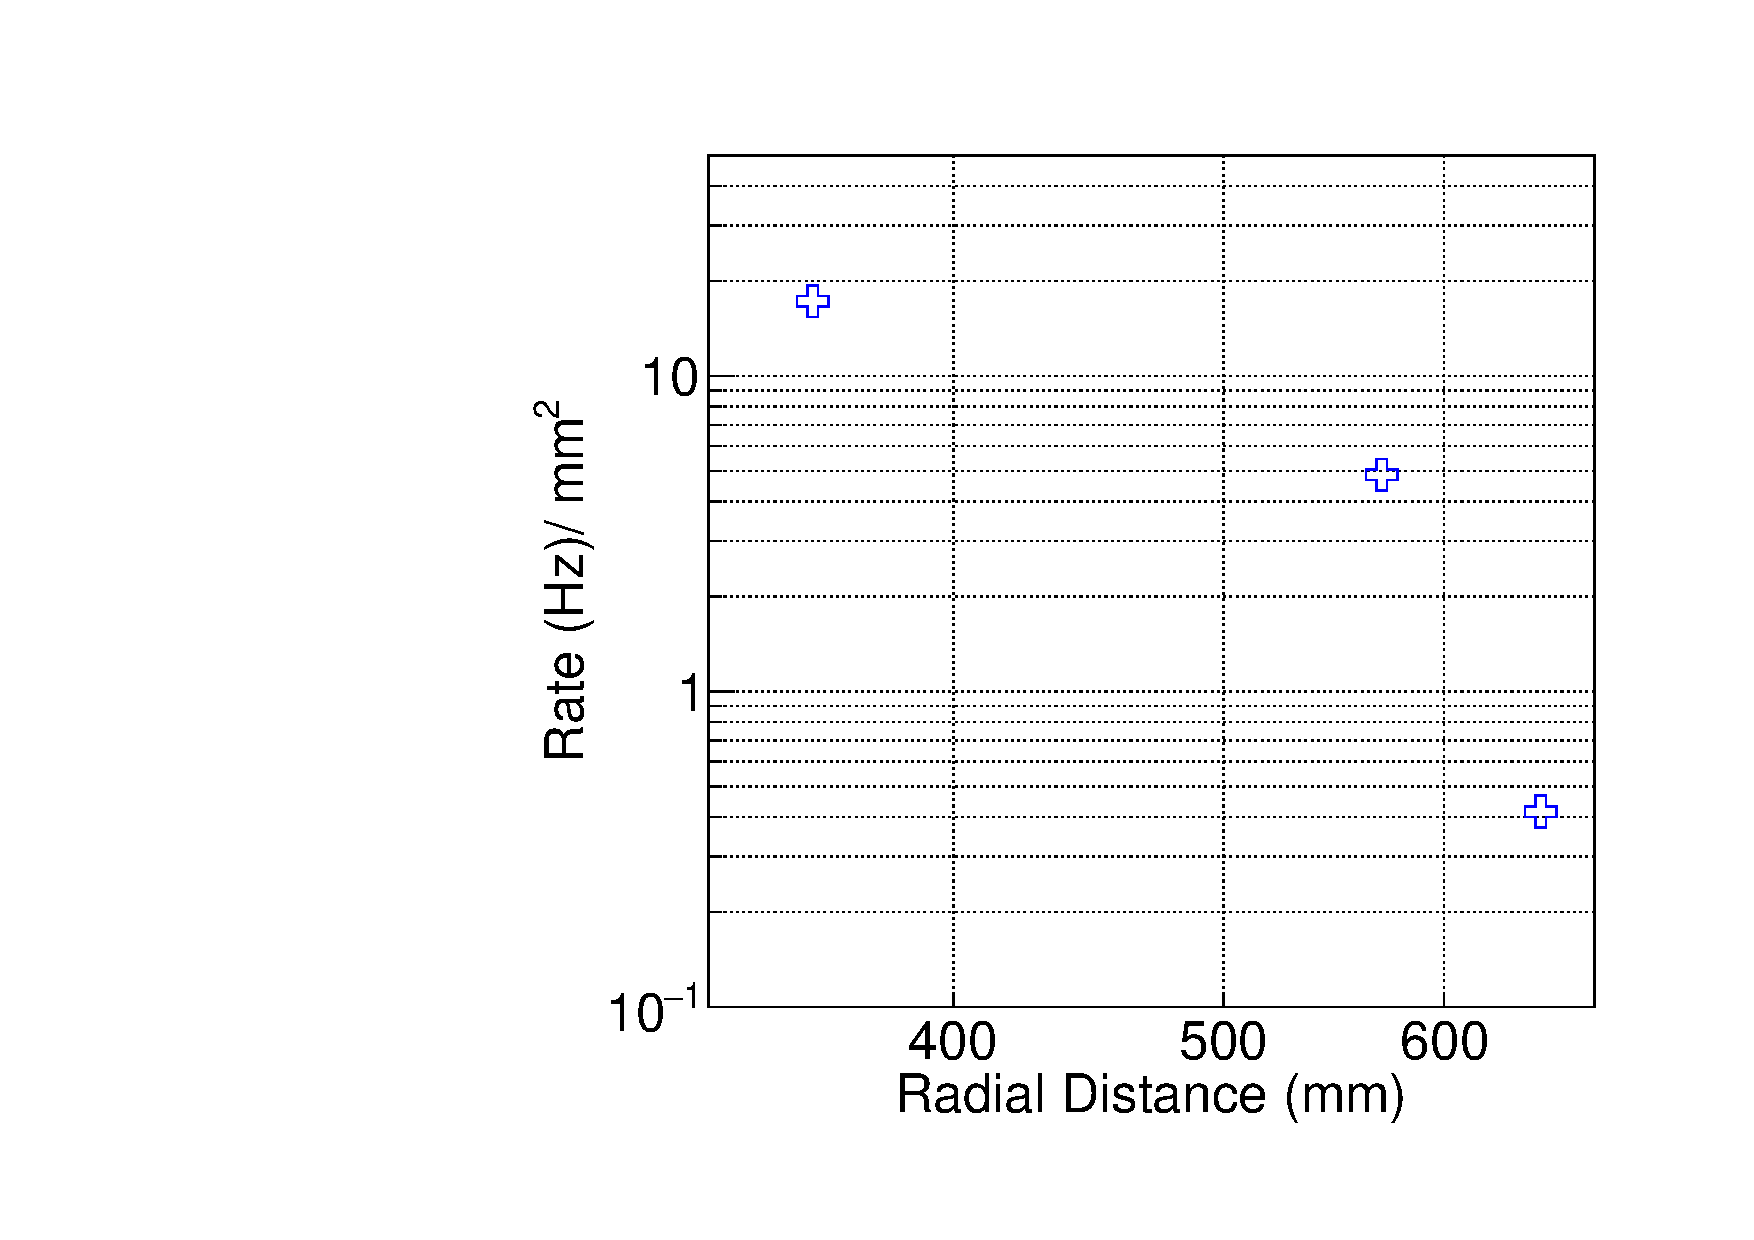
\includegraphics[width=4cm]{plots/rate_vs_radius} 
\caption{X-ray
interaction rates in LYSO scintillator inside and outside COBRA magnet
(left) and normalized interaction rate as a function of radial
distance (right).} \label{fig:absorption} 
\end{figure}  


%\subsection{Scan Summmary}
The collimator projects a thin beam on the inner face of the cryostat
fully covering two MPPCs simultaneously in the long direction.  The Z
and $\phi$ coordinates of the MPPCs are scanned separately, each using
the long-edge of the collimated beam in the vertical and horizontal
orientations respectively. Data is collected with the scanning step of
1~mm (0.08~deg) in Z ($\phi$) direction.  Increase in the material
cross-section outside the axially central region ($|$Z$|>$120 mm)
causes enhanced absorption of the X-rays making the calorimeter nearly
opaque to the X-ray scan (Figure~\ref{fig:ratevsz}).  Hence, the scanning
region is restricted in $|$Z$|<$120~mm and covers the entire range in
$\phi$, $120\degree<\phi<\,240\degree$.  In 2017, the full set of the
accessible MPPCs about 46\% (1900 of 4092) were scanned; a subset of
these, about 700, were scanned again in 2018.

\begin{figure}[] 
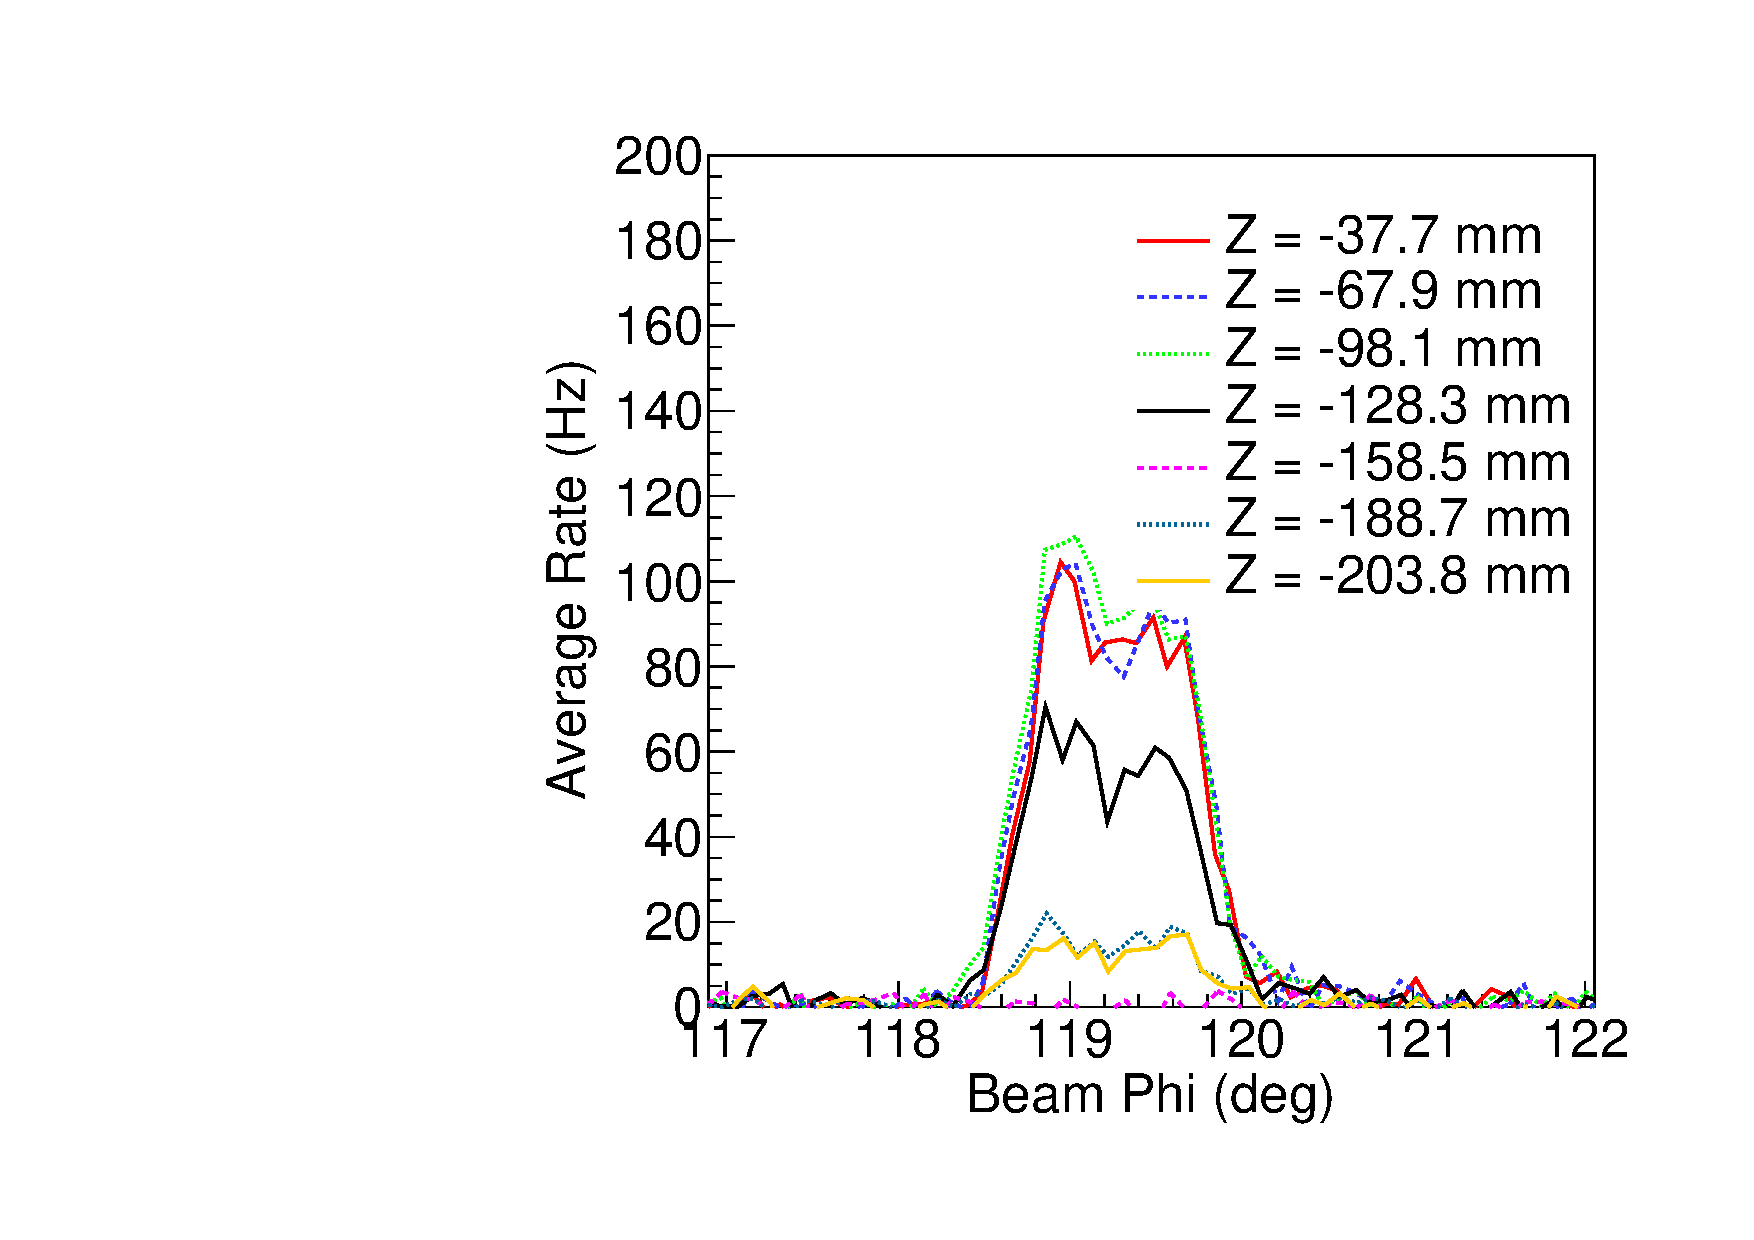
\includegraphics[width=4cm]{plots/xray_vs_Z}
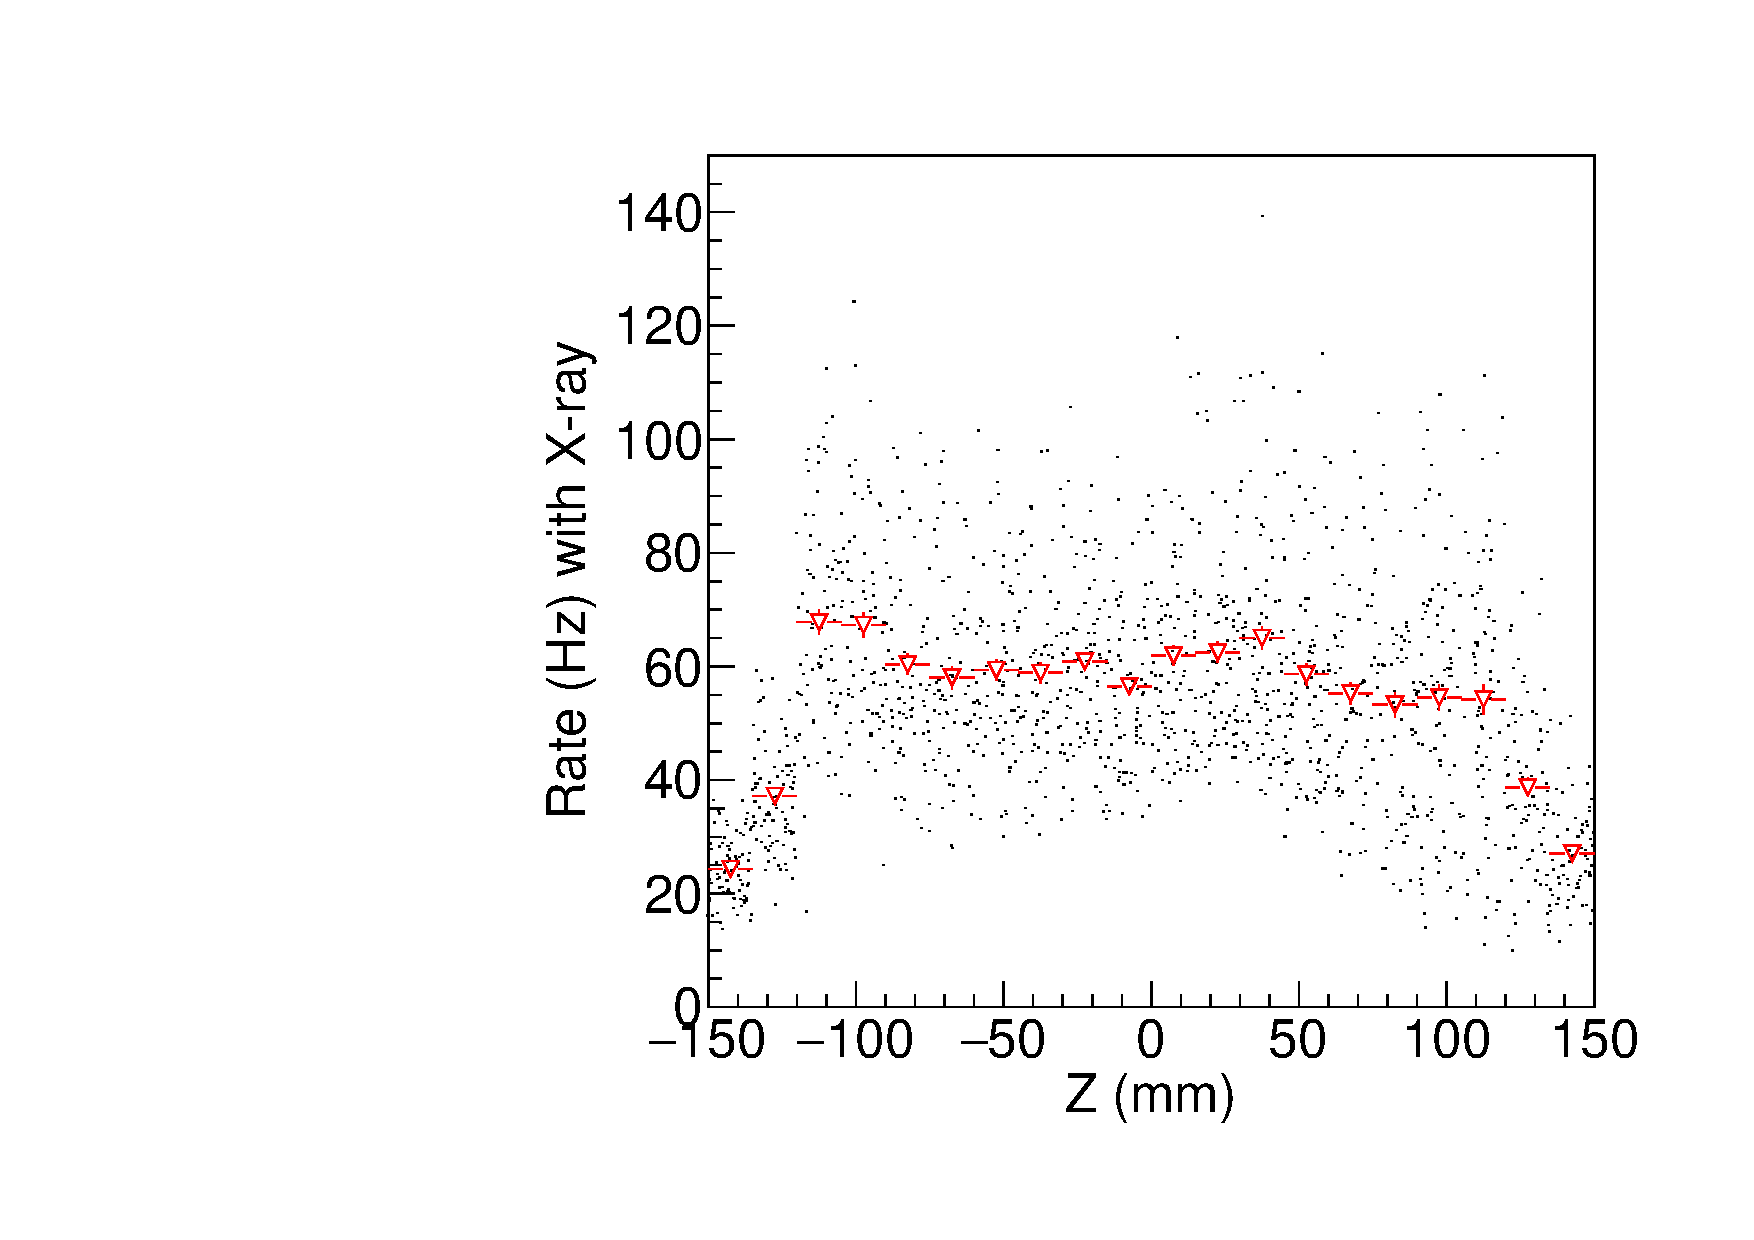
\includegraphics[width=4cm]{plots/csig_z_phiscan} \caption{Drop in
observed X-ray interactions as a function of axial (Z)  location.}
\label{fig:ratevsz} 
\end{figure}  


%%\begin{figure}[]
%%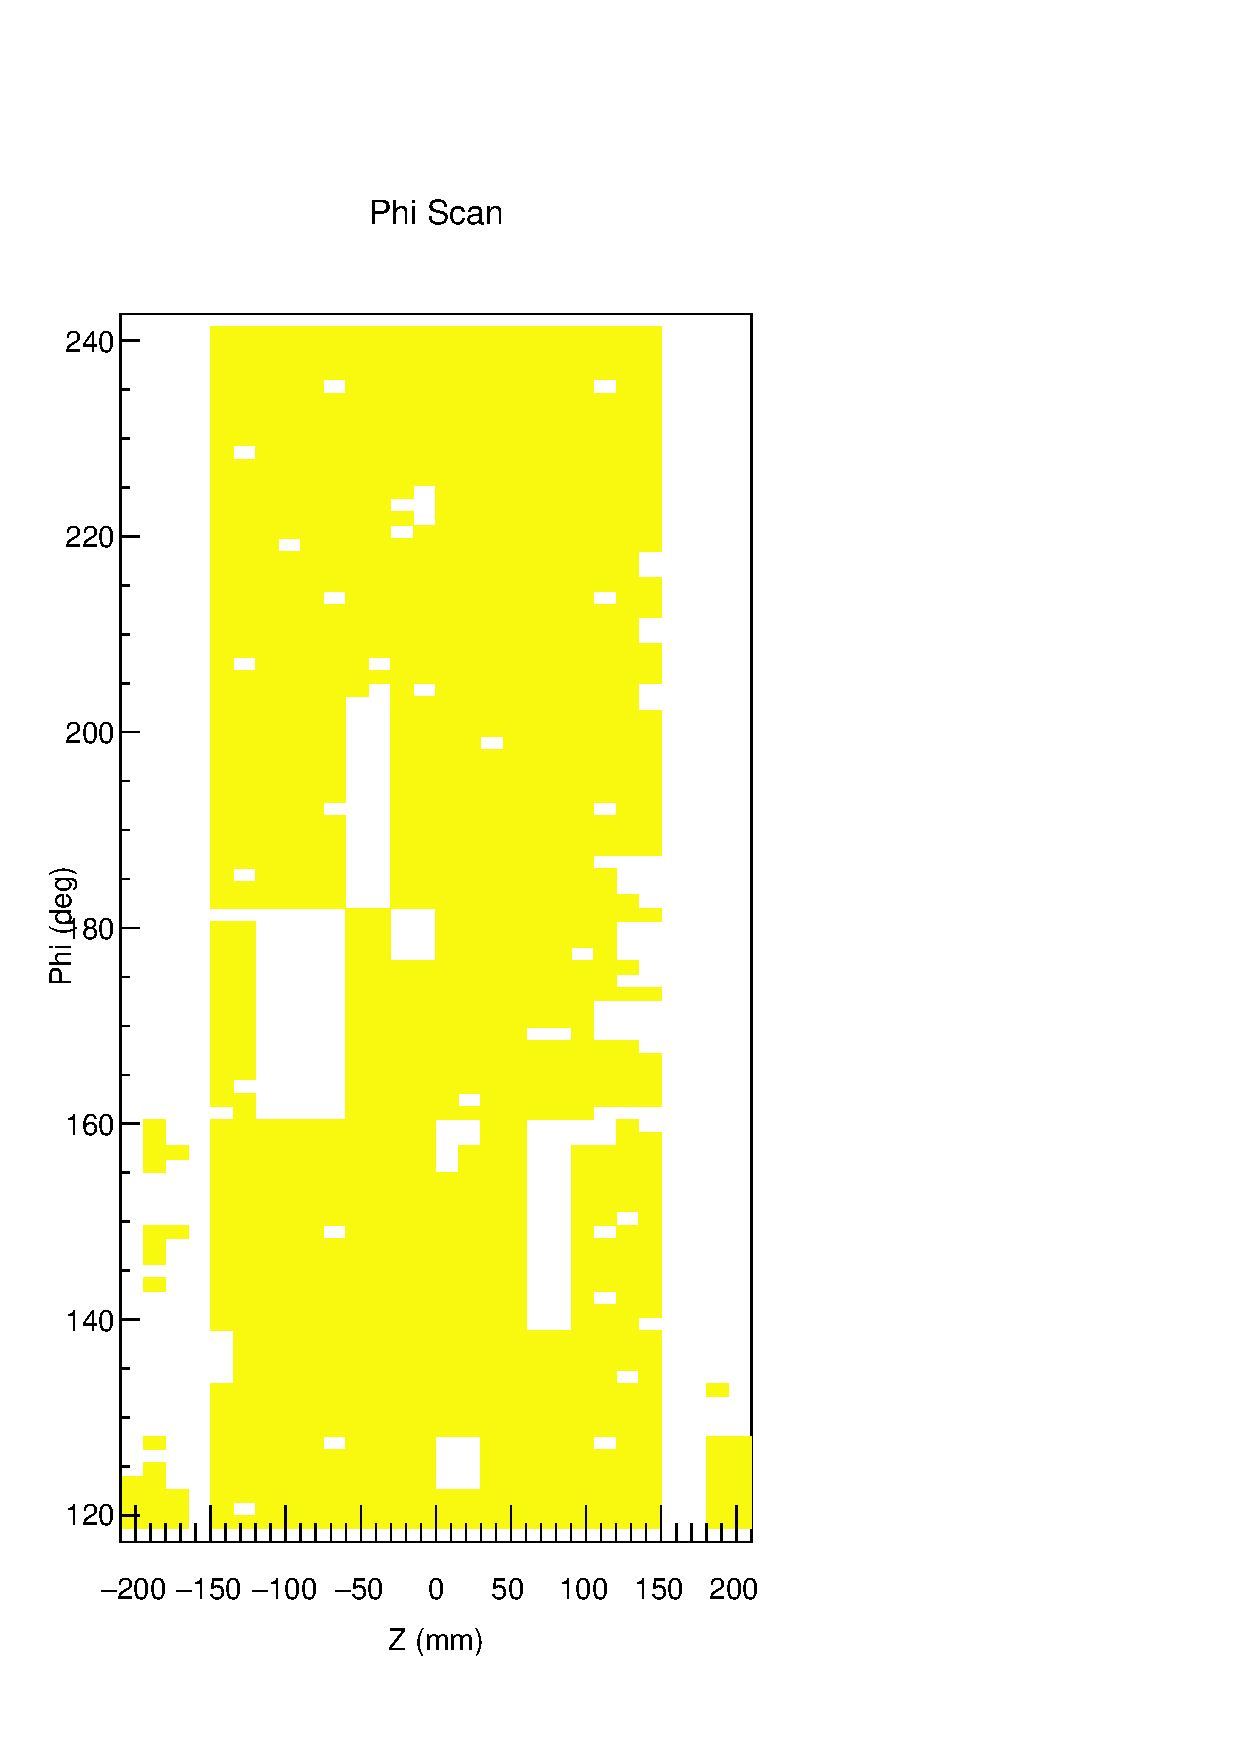
\includegraphics[width=7cm]{plots/c2_phi}
%%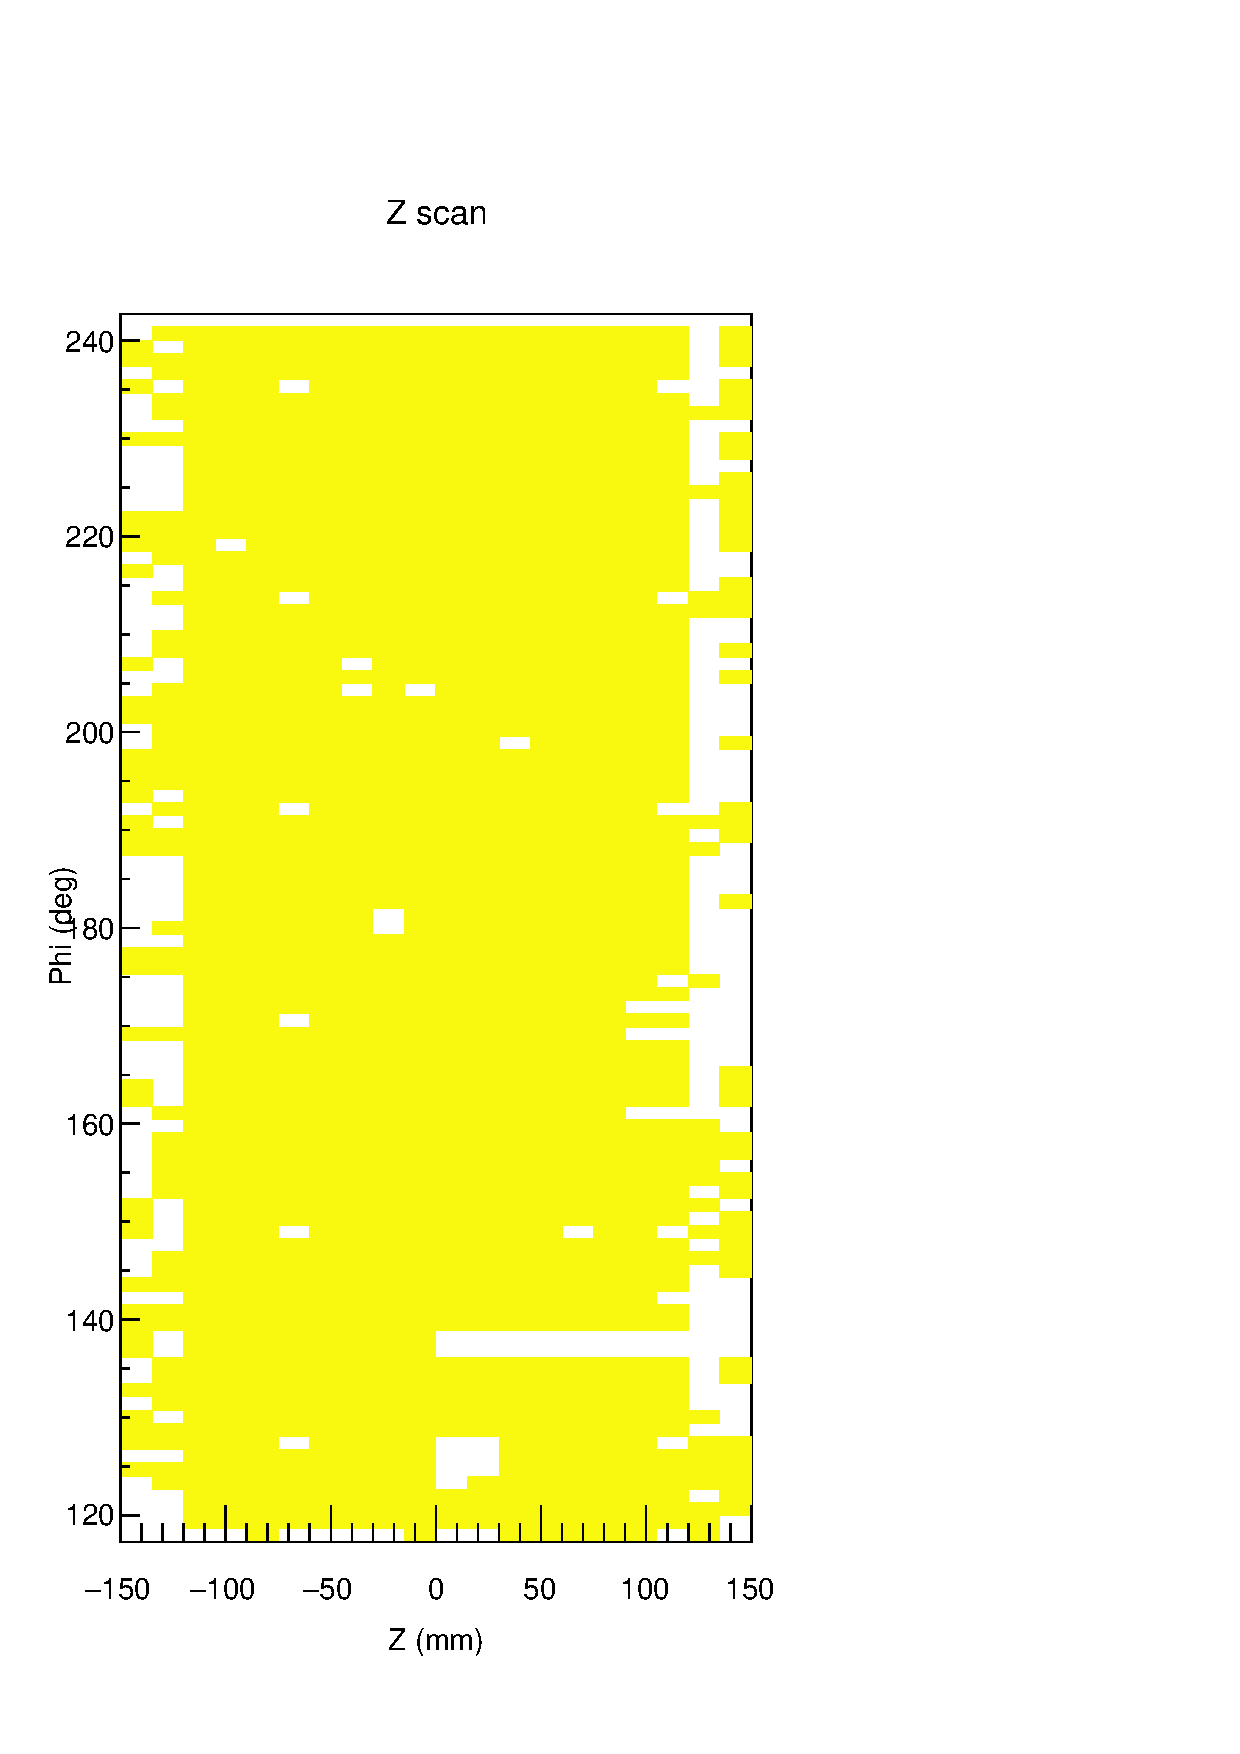
\includegraphics[width=7cm]{plots/calc-all}
%%\caption{Scanned MPPCs for $\phi$ and Z coordinates after quality cuts.}
%%\label{fig:scanmap}
%%\end{figure}  


